\section{Accesso ai file}
L' accesso ai file su UNIX/Linux è di tipo sequenziale, per ogni file aperto abbiamo un file descriptor che per l' utente è costituito da un intero ma nel sistema operativo è l' indice di un elemento nella tabella dei file aperti di processo.
Ogni entrata è un file descriptor che punta ad una entrata nella tabella dei file aperti di sistema in cui ogni entrata è un I/O pointer che a sua volta riferisce una entrata nella tabella dei file attivi che contiene un i-node.

Ogni processo che lancia una open quindi causa la creazione di una entrata nella tabella dei file di processo e di una entrata nella tabella dei file di sistema, tuttavia entrambe punteranno allo stesso i-node.

IO-pointer ed i-node permettono di trovare l' indirizzo fisico in cui effettuare la prossima lettura/scrittura.

NB: STDIN, STDOUT, STDERR sono descrittori aperti di default al momento dell' esecuzione del programma.

\subsection{File descriptors e fork}
Se un processo con dei file aperti esegue una fork il figlio eredita i file aperti, si duplicano quindi le user structure con tutti i file descriptor ma entrambi punteranno allo stesso elemento nella tabella dei file aperti di sistema:
\begin{figure}[H]
    \centering
    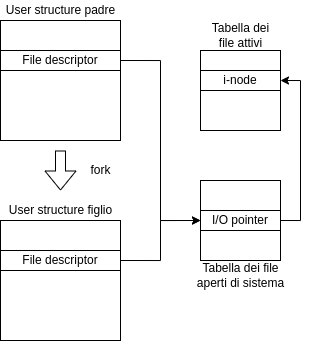
\includegraphics[width=200px]{images/5L_Accesso_ai_file/file_descritor_and_fork.png}
\end{figure}
Quando uno dei due legge muove l' I/O pointer anche all' altro!

\subsection{Primitive per l' accesso ai file}
\subsubsection{open()}
\begin{verbatim}
    int open(const char* path, int flags)
\end{verbatim}
\begin{itemize}
    \item percorso del file da aprire
    \item Modalità di accesso:
    \begin{itemize}
        \item \verb{O_RDONLY{
        \item \verb{O_WRONLY{
        \item \verb{O_RDWR{
    \end{itemize}
    sono macro che si trovano in \verb{fcntl.h{.
    Più macro possono essere messe assieme utilizzando l' OR delle due macro.
\end{itemize}
All' apertura l' IO pointer viene posizionato all' inizio del file a meno che non si sia specificato l' accesso come \verb{O_APPEND{, in tal caso viene inizializzato alla fine del file.
Ritorna un intero che è il file descriptor.

\subsubsection{read()}
\begin{verbatim}
    ssize_t read(int fd, void* buffer, size_t count)
\end{verbatim}
\begin{itemize}
    \item file descriptor dal quale leggere
    \item buffer sul quale scrivere i valori letti
    \item quantità dei byte da leggere
\end{itemize}
Ritorna la dimensione effettivamente letta e trasferita nel buffer oppure un numero negativo in caso di errore.

\subsubsection{write()}
\begin{verbatim}
    ssize_t write(int fd, const void* buf, size_t count)
\end{verbatim}
\begin{itemize}
    \item file descriptor sul quale scrivere
    \item buffer dal quale leggere i dati da scrivere
    \item quantità di byte da scrivere
\end{itemize}
Ritorna il numero di byte effettivamente scritti, oppure un numero negativo in caso di errore.

\subsection{Comunicazione tramite pipe}
L' astrazione delle pipe è omogenea rispetto alla gestione dei file, quindi creando una pipe quello che si vede è un normale file descriptor.
A ciascun estremo è associato un file descriptor ed i problemi di sincronizzazione sono risolti dalle primitive read/write in quanto bloccanti.

I figli ereditano gli stessi file descriptor e possono utilizzarli mentre per la comunicazione tra processi che non sono nella stessa gerarchia si utilizzano i fifo (named pipe) o i socket.

\subsubsection{pipe()}
Per generare una pipe si usa l' omonima primitiva:
\begin{verbatim}
    int pipe(int fd[2])
\end{verbatim}
\begin{itemize}
    \item vettore di due interi in cui al primo posto verrà inserito il file descriptor della pipe in lettura e nella seconda posizione verrà inserito il fd dell' estremo per la scrittura
\end{itemize}
Ritorna zero se ha successo, -1 altrimenti.




